\documentclass[12pt, a4paper, oneside]{article}
\usepackage{amsmath, amsthm, amssymb, bm, graphicx, hyperref, mathrsfs,color}

\begin{document}

%\maketitle
\begin{center}
	\rule{\textwidth}{1pt}\par
	\vspace{5mm}
	{\large\scshape UM-SJTU Joint Institute}\\[\baselineskip]
	{\large\scshape Physics Laboratory}\\
	(Vp141)
	\rule{\textwidth}{1pt}\par
	\vspace{4cm}
	{\large\scshape Laboratory Report}\\[\baselineskip]
	{\large\scshape Excercise 5}\\[\baselineskip]
	{\large\scshape Damped and Driven Oscillations\\Mechanical Resonance}\\[\baselineskip]
\end{center}
\vspace{7cm}

\begin{tabular}{lll}
	Name:Kaixuan Wang & ID:523370910219 & Group:1 \\
	Date: {\today}    &                 &         \\
\end{tabular}


\rightline{\footnotesize[rev4.1]}
\pagebreak

\section{Introduction}
% \textcolor{blue}{This part should include a brief description of the experiment: its objectives, underlying physical model and phenomena, and equations that you will use in
% 	your calculations. It may be a bit longer than that below, but you should not simply copy the lab manual or quote long passages from textbooks.}
\indent

The objective of this exercise is to understand the physics of alternating-current circuits, in particular the process of charging
and discharging of capacitors, the phenomenon of electromagnetic induction in inductive elements, and other dynamic processes in $RC,
RL$, and $RLC$ series circuits. This experiment also measures the amplitude-frequency and the phase-frequency characteristics of $RC,
RL$, and $RLC$ series circuits.

\section{Experimental setup}
\indent
\subsection{Equipments used in the experiment}
\indent

Three basic elements of electric circuits include resistors, capacitors, and inductors. In this experiment, we will be using a alternating
electric power source with a fixed frequency of 1000Hz, an inductor with a fixed inductance of 0.01H, 
a capacitor with a fixed capacitance of about 125nF, a fixed resistance of 100 $\Omega$, and fixed electromotive force of 4 Vpp. 

\subsection{Measurements used in the experiment}
\indent

In the first two circuits, i.e. the $RC, RL$ circuits, our objective is to measure the half life of the capacitor's charging and 
discharging. During a complete period, the capacitor will first be charged and then be discharged, which means its voltage will first 
reach its peak and then drop back to zero. Here, the half life refers to the time it takes for the capacitor's voltage to increase 
a half from 0 or drop a half from its peak. The equations for calculating the voltage of the capacitor is shown as following:

\begin{equation}
	RC \frac{dU_c}{dt} + U_c = E
\end{equation}

\begin{equation}
	RC \frac{dU_c}{dt} + U_c = 0
\end{equation}

We will first obtain the measured half life using an oscilloscope, then calculate the theoretical value of the half life 
using the following equations:
\begin{equation}
	T_{1/2}=\tau ln(2)=RC*ln2\\
	\label{eq_RC}
\end{equation}

\begin{equation}
	T_{1/2}=\tau ln(2)=\frac{L}{R}*ln2\\
	\label{eq_RL}
\end{equation}

After obtaining both the experimental and the theoretical values of the half life, we can compare them and derive some onclusions. 

For the $RLC$ circuits, it becomes a bit more complicated. We will first also deal with the half life. Here, we introduce a new 
constant $\beta$ which is given by:
\begin{equation}
	\beta=\frac{R}{2L}
\end{equation}
This constant has the following relationship to the half life with:
\begin{equation}
	\beta T_{1/2}=1.68
\end{equation}
and we also have:
\begin{equation}
	\tau=\frac{1}{\beta}=\frac{T_{1/2}}{1.68}
	\label{eq_RLC}
\end{equation}
With all these relationships, we should also come up with a theoretical and experimental value of the time constant $\tau$. We then
compare them and draw some conclusions. 

After that, we pay attention to the resonance in the $RLC$ circuit. Resonance happens in the $RLC$ circuit only when the 
frequency of the power satisfy the following equation:
\begin{equation}
	f=\frac{1}{2\pi\sqrt{LC}}
	\label{eq_fre}
\end{equation}
We also would like to calculate the quality factor $Q$ of the circuit using the following equation:
\begin{equation}
	Q=\frac{1}{\omega_0 RC}
	\label{eq_Q}
\end{equation}
where $f_0$ is the resonance frequency, and $f_1$ and $f_2$ are two frequencies that satisfy: $I(f_1)=I(f_2)=I_m/\sqrt{2}$.

\section{Measurements and Results}
\subsection{RC circuit half life}
\indent

Below is the data table of the RC circuit:
\begin{figure}[htbp]
	\centering
	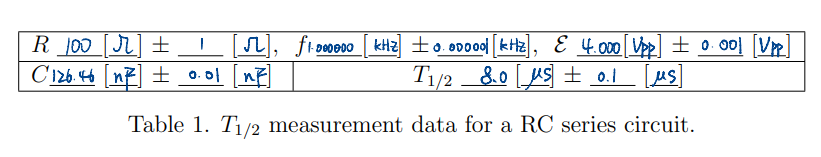
\includegraphics[width=0.9\textwidth]{C1.png}
	\caption{Data table for RC circuit}
\end{figure}
From the data collected we see that the experimental value of the half life is $8.0\mu s$, which means the experimental time constant
$\tau$ is about $11.542\mu s$. The theoretical value can be derived using the equation \ref{eq_RC}, and we have the result that is should
be $12.646\mu s$. 

\subsection{RL circuit half life}
\indent

Above is the data table of the RC circuit:
\begin{figure}[htbp]
	\centering
	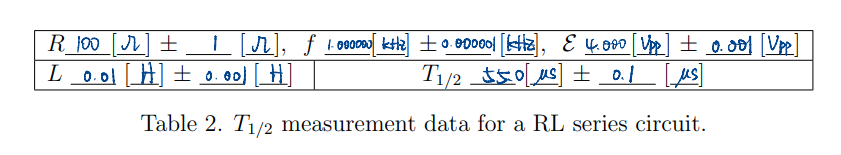
\includegraphics[width=0.9\textwidth]{C2.png}
	\caption{Data table for RL circuit}
\end{figure}

From the data collected we see that the experimental value of the half life is $55.0\mu s$, which means the experimental time constant
$\tau$ is about $79.348\mu s$. The theoretical value can be derived using the equation \ref{eq_RL}, and we have the result that is should
be $81\mu s$. 

\subsection{RLC circuit half life}
\indent

Below is the data table of the RLC circuit:
\begin{figure}[htbp]
	\centering
	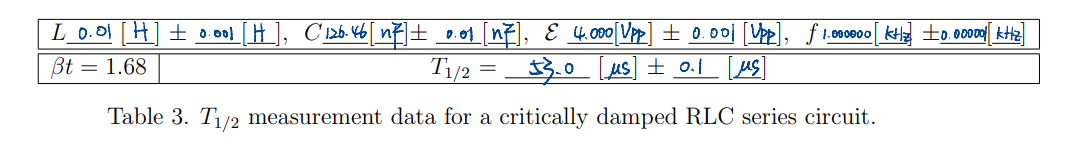
\includegraphics[width=0.9\textwidth]{C3.png}
	\caption{Data table for RLC circuit}
\end{figure}

From the data collected we see that the experimental value of the half life is $353.0\mu s$ (here should be 
a mistake: missing a 3 for the first digit), which means the experimental time constant
$\tau$ is about $210\mu s$. The theoretical value can be derived using the equation \ref{eq_RLC}, and we have the result that is should
be $200\mu s$. 

\subsection{RLC circuit resonance frequency}
\indent

Below is the data table of the RLC resonance circuit:
\begin{figure}[htbp]
	\centering
	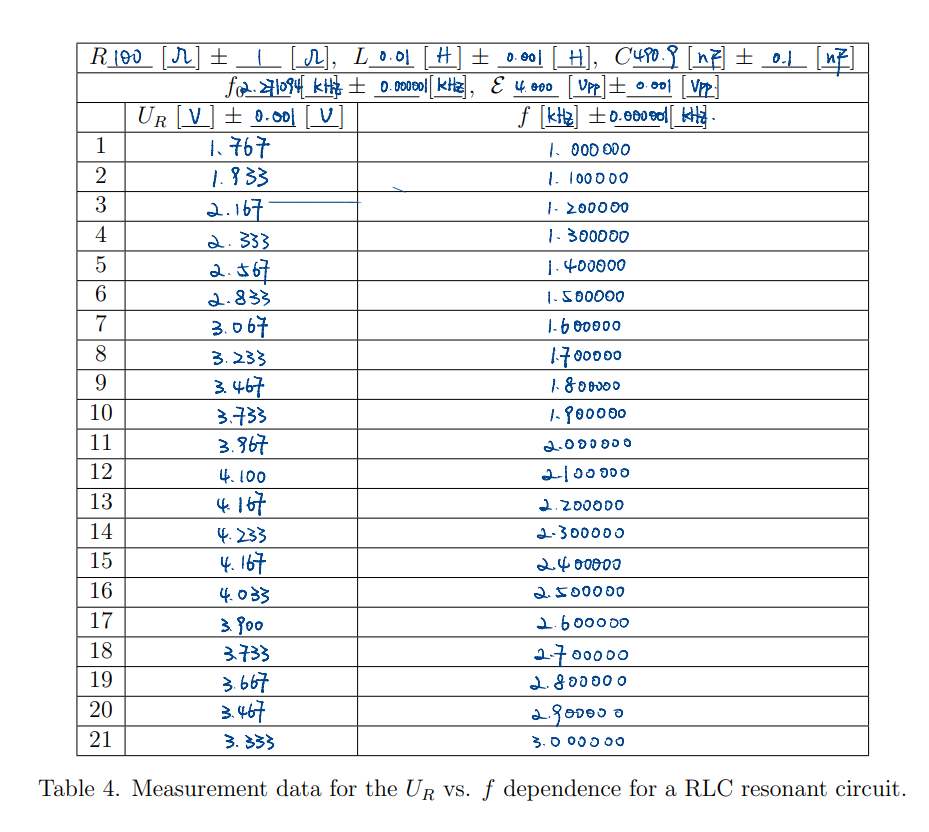
\includegraphics[width=0.9\textwidth]{C4.png}
	\caption{Data table for RLC circuit}
\end{figure}

We see from the data table that the theoretical value of $f_0$ is 2271.064 Hz, which is derived using the equation \ref{eq_fre}. 
Here we need 2 plots: I vs f and $\varphi$ vs f. I and $\varphi$ are given using the following 
equations: 
\begin{equation}
	I=\frac{U_R}{R}
\end{equation}

\begin{equation}
	\varphi=tan^{-1}(\frac{2\pi fL-\frac{1}{2\pi fC}}{R})
\end{equation}
After calculation, we have the following 2 graphs:

\begin{figure}[htbp]
	\centering
	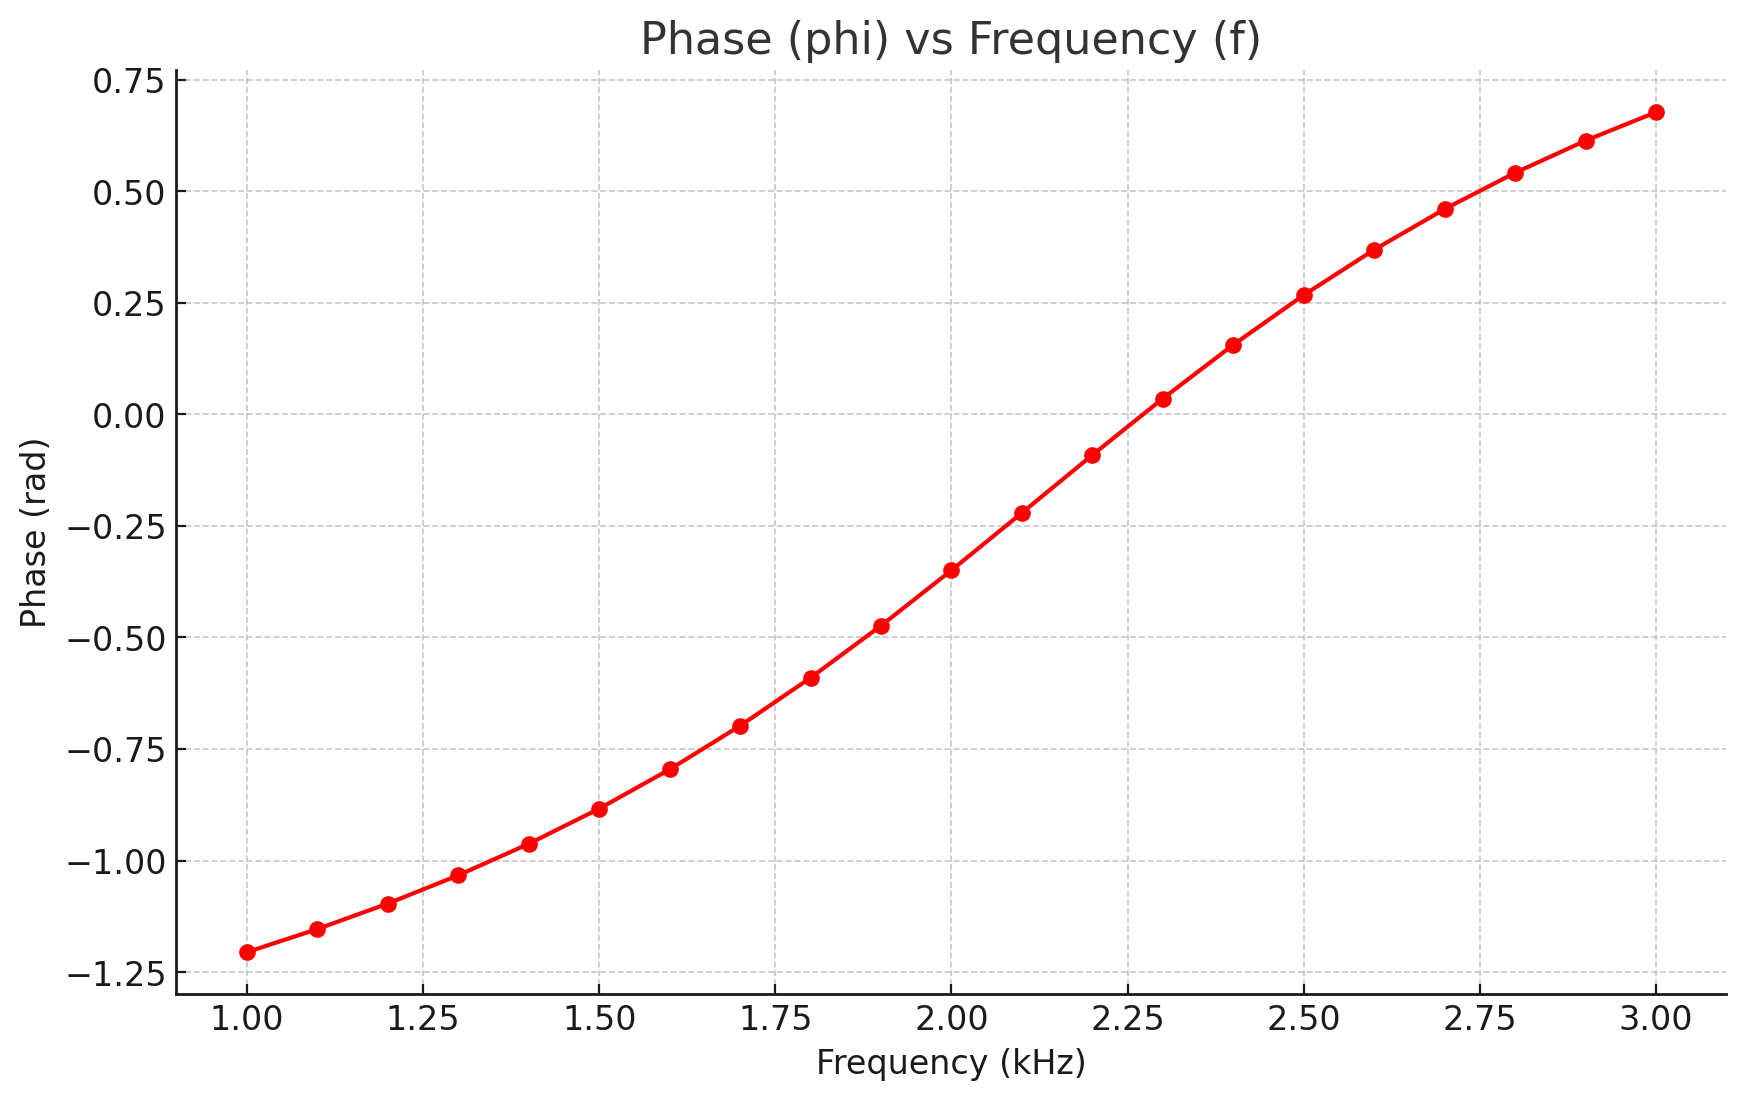
\includegraphics[width=0.9\textwidth]{C5.png}
	\caption{Data table for RLC circuit}
\end{figure}

\begin{figure}[htbp]
	\centering
	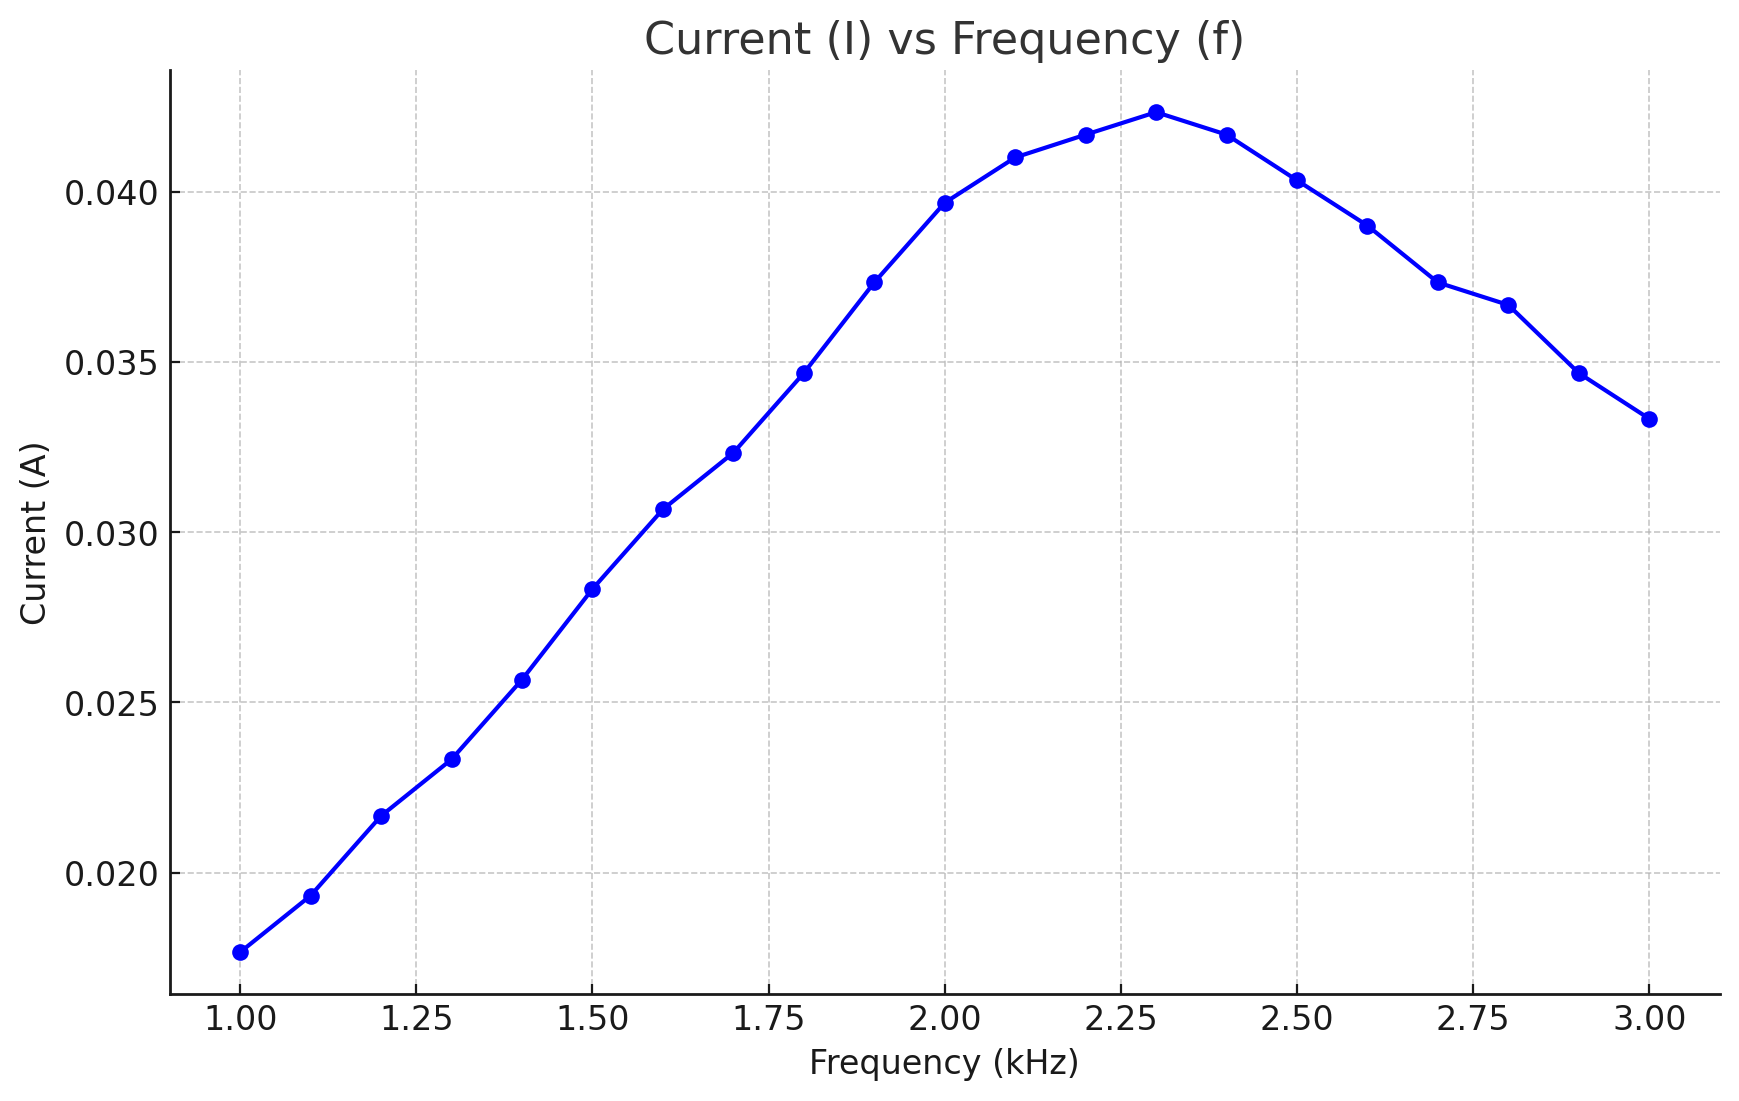
\includegraphics[width=0.9\textwidth]{C6.png}
	\caption{Data table for RLC circuit}
\end{figure}

From the figures we can see that the resonance frequency is about 2.27-2.28kHz. And for the 
quality factor, we use equation \ref{eq_Q} and get Q to be about 1.46

\section{Conclusions and discussion}
\indent

As mentioned above, the objective of this experiment is to check the theories about $RC,RL$ and $RLC$ circuits to deepen our understanding, and have a better understanding 
about the theories. In the RC circuit and the RL circuit, both time constants,
the theoretical and the experimental ones, are very close to each other. If we 
calculate the mistake percentage, we will see that they are all smaller than the 
10\% expectation and is within our tolerance. For the RLC circuit, there should 
be a little mistake in the data table as mentioned before, which is missing a 3 for 
the most significant digit, but after fixing this little mistake, the value is
also within the range of 10\%, so it is also acceptable. 
Then there is the resonance frequency derived in the RLC circuit. The theoretical
resonance frequency of this circuit is 2271.064Hz, and the experiment data reveals
the experimental resonance frequency to be about from 2.27kHz to 2.28kHz, which is 
accurate enough. 

However, although some results are within our tolerance of error, the percentage
of error is a bit high, or in other words close to the boundary of tolerance. We propose
that these mistakes may have originated from the huge amount of usage of the equipments.
In the first 2 experiments, the capacity is expected to be at 100nF, but the result 
of measurement is 126.46nF, and we see that the error is over 25\%. So we guess
that this is a reasonable explanation of the errors. 

\section{Works cited}
Department of Physics, Shanghai Jiaotong University, Exercise 5 (RC, RL, and RLC Circuits) - lab manual [rev. 2.6], 2024\\
Python Software Foundation. (2020). Python Language Reference, version 3.9. Available at http://www.python.org\\
\\
All the figures displayed in the article (excluding the appendix) are given using Python 3.9.
\pagebreak
\appendix
\section{Datasheet}

\begin{figure}[htbp]
	\centering
	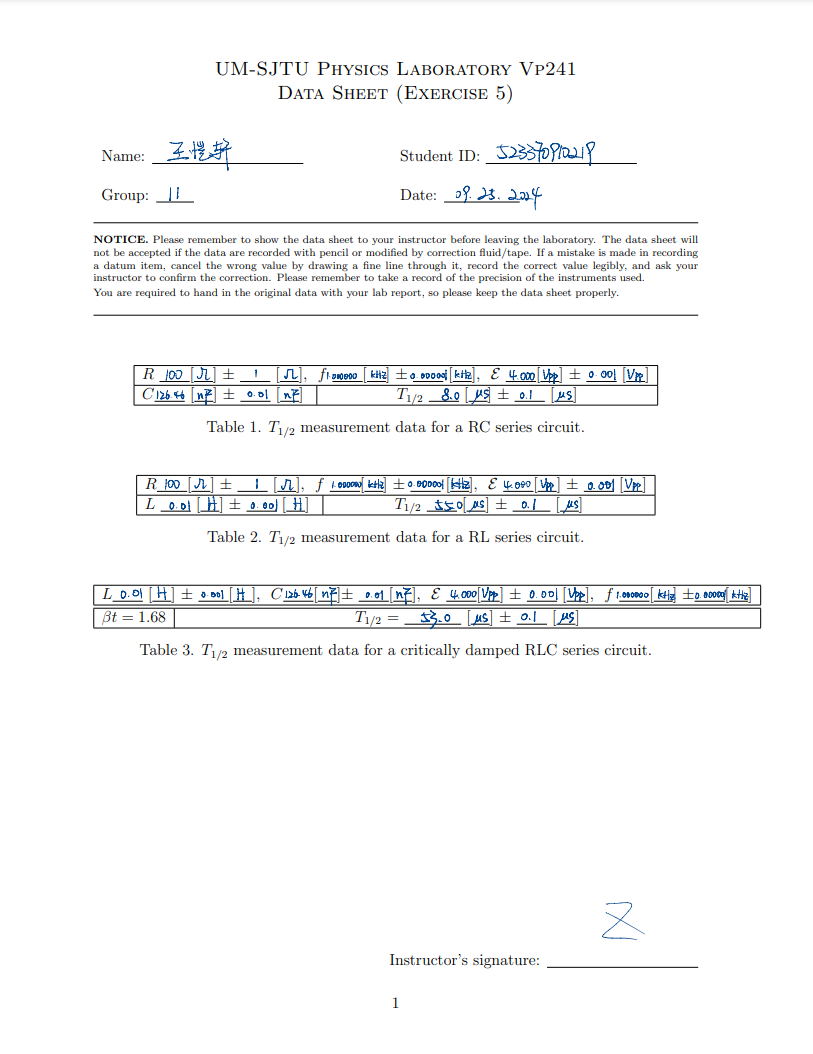
\includegraphics[width=0.75\textwidth]{D1.png}
	\caption{Datasheet 1}
\end{figure}

\begin{figure}[htbp]
	\centering
	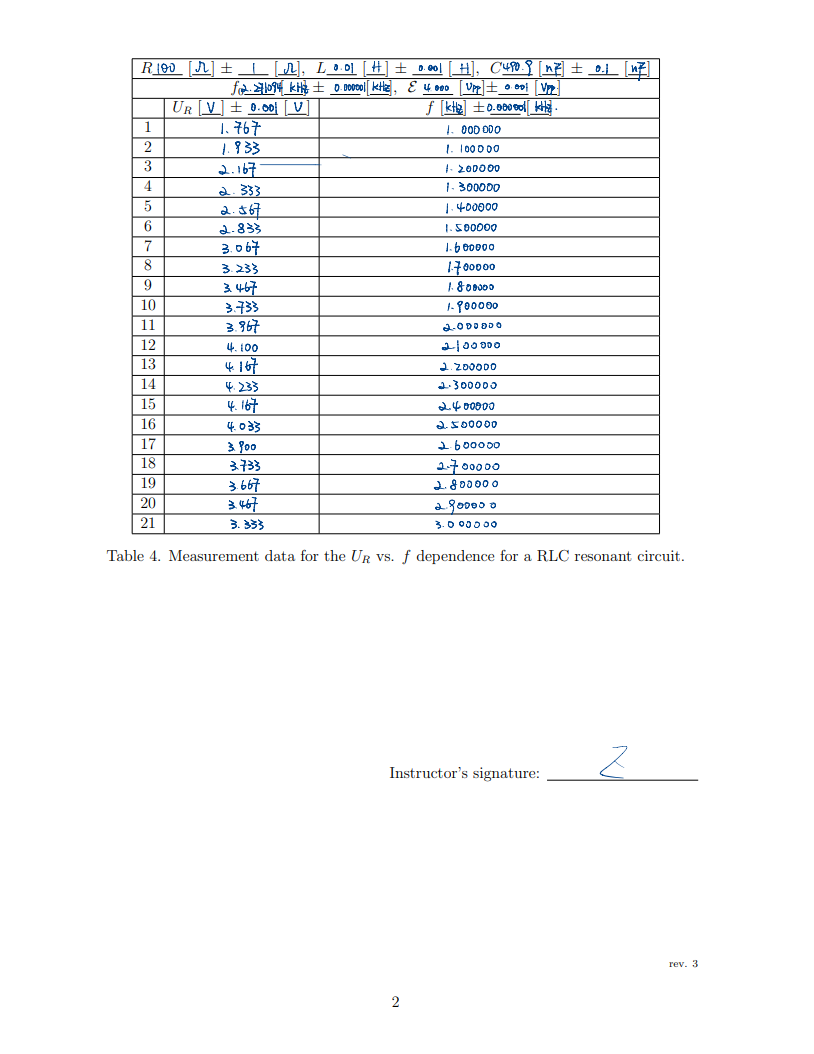
\includegraphics[width=1.0\textwidth]{D2.png}
	\caption{Datasheet 2}
\end{figure}

%\textcolor{blue}{Please remember to attach the original data sheet signed by your instructor.}
\end{document}